\documentclass{micart}

\usepackage{array,booktabs} % For nice tables
\usepackage{amsmath,amssymb} % For nice maths
\usepackage{stfloats} % For putting double column floats on bottom of page
\usepackage{hyperref}
\usepackage{color}
\usepackage{flushend}
\definecolor{darkgreen}{rgb}{0,0.75,0}

\hypersetup{
	pdfauthor={Geir Hovland, P�l Johan From, Lars Imsland, Jostein Bakkeheim, Morten Hovd},
	pdftitle={Sample article for Modeling, Identification and Control based on pdfLaTeX},
	pdfkeywords={MIC,pdflatex,vector graphics},
	pdfsubject={MIC Journal Article},
	colorlinks=true,
	citecolor=darkgreen,
	urlcolor=darkgreen,
	pdfstartview=Fit,
	pdfpagelayout=SinglePage,
	pdfcreator=pdflatex,
	pdfproducer=pdflatex}

\newcounter{tempeqncnt} % Counter for temporarily saving equation number

\firstpage{1}    % Set page number for first page
\MICvolume{31}   % Volume number
\MICissue{1}     % Issue number
\MICyear{2010}   % Year
\MICdoi{mic.2010.1.1}   % Year, issue, paper number in issue
\shorttitle{Hovland et.al., ``Sample article for MIC based on pdfLaTeX''}

\begin{document}

\title{Sample article for Modeling, Identification\\ and Control based on pdfLaTeX}

% The optional argument to \author points to the \address, see below.
% The last argument, in this case {1}, turns on the superscript for the authornames.
% Use {0} to turn this off. The same applies to \address
% In general, when there is only one address, then {0} should be used, otherwise {1}
% {2} is the same as {0], except that the address is centered.

\author[UiA]{G. Hovland}{1}
\author[IKT]{P.J. From}{1}
\author[SINTEF]{L. Imsland}{1}
\author[IKT]{J. Bakkeheim}{1}
\author[IKT]{M. Hovd}{1}

\address[UiA]{Mechatronics Group, University of Agder, N-4898 Grimstad,
   Norway. E-mail: \textsf{geir.hovland@uia.no}}{1}

\address[IKT]{Department of Engineering Cybernetics, Norwegian
   University of Science and Technology, N-7491 Trondheim, Norway.
   E-mail: \textsf{\{from,Jostein.Bakkeheim,Morten.Hovd\}@itk.ntnu.no}}{1}

\address[SINTEF]{SINTEF ICT, N-7465 Trondheim,
   Norway. E-mail: \textsf{Lars.Imsland@sintef.no}}{1}

\begin{abstract}
  This article contains a sample article file
  for Modeling, Identification and Control, based on the class file
  \textsf{micart.cls}. The article contains hints on how to produce
  articles on PDF format including vector graphics using pdfLaTeX.
\end{abstract}

\begin{keywords}
  Choose three to five representative keywords
\end{keywords}

\maketitle

\section{Introduction}
\label{sec:intro}

This is a sample article file for Modeling, Identification and
Control, illustrating the use of the class file \textsf{micart.cls}.
This class file is built upon the class file \textsf{scrartcl.cls}
from the KOMA-script bundle, which replaces the standard latex classes
(article, book, report), being inspired by european typographical
standards.

The traditional \LaTeX \ compiler generates a Postscript file and all figures used in
the article must be saved as Encapsulated Postscript. To generate the final PDF file,
a Postscript to PDF converter is needed.

pdfLaTeX is a variant of the \LaTeX \ family of compilers which generates an output file
directly to the PDF format. By using pdfLaTeX the final conversion step from Postscript
is avoided. pdfLaTeX can import many different types of image files, such as JPG, PNG and
PDF. However, the formats JPG and PNG store images as bitmaps, and the quality of the images
are lower compared to vector graphics and the file size is also normally larger. MIC strives
to keep the PDF file size as low as possible and the figure quality as high as possible,
hence using figures with vector graphics is strongly encouraged. From May 2009, MIC is again available in
printed versions. To produce the printed version, the page size is reduced from A4 by about 20\%.
Hence, to get the best quality in the printed version, the use of vector graphics is strongly
recommended.

% The double column equation must be placed in a float on the page
% before it should appear!
\begin{figure*}[b!]
  \normalsize
  \setcounter{tempeqncnt}{\value{equation}} % Save the equation number
  \setcounter{equation}{1} % Manually set the double column equation
                           % number to one less than it should be
  \centering
  \hrulefill % Separate with a line
  \begin{align}\label{eq:floateqn}
    \tilde{V}(x(\infty),\eta(\infty)) - \tilde{V}(x(t_i),\eta(t_i))
    \leq -\int_{t_i}^{\infty}\!\!\!\!\!\!F(x(\tau),u(\tau;\hat
    x_0))d\tau - \int_{t_i}^{\infty} \!\!\!\! \kappa \|\eta(\tau)\| d
    \tau.
  \end{align} 
  \hrulefill % Separate with a line
  \setcounter{equation}{\value{tempeqncnt}} % Restore equation counter
%  \vspace*{4pt} % Add some space
\end{figure*}

Many programs can generate figures on vector graphics format. The most
common example is Matlab and the command 'print -deps'. The print command
works for 2D and 3D plots as well as Simulink block diagrams. One excellent
drawing program for \LaTeX \ is WinFig (or XFig), which can
save vector graphic figures both as Encapsulated Postscript or directly
as native \LaTeX \ figures. The latter approach also allows \LaTeX \ equations
to be used inside the figures. Another option to generate vector graphics is to use
Microsoft Visio or Microsoft Powerpoint by saving to the Windows Metafile format EMF.

To use vector graphics generated as Encapsulated Postscript directly with
pdfLaTeX, these figures must first be converted to vector graphics PDF figures.
This conversion can be made using Ghostview (File - Convert - pdfwrite). Otherwise,
the PDF figures are imported into pdfLaTeX using the {\tt includegraphics} command
in exactly the same way as EPS files using the traditional \LaTeX \ compiler.
The EMF format can be converted to EPS (for example by the freeware EMF2EPS by Dirk
Struve, 1999) and finally to vector graphic PDF by Ghostview. To crop graphics
from EPS files, it may be necessary to first perform 'PS to EPS' in Ghostview followed
by 'Media - User Defined (Width and Height)' and finally 'File - Convert -
pdfwrite - Properties - Page Offsets'.

Another advantage of using pdfLaTeX compared to the traditional \LaTeX compiler, is the added options of the {\tt href} package.
The {\tt href} information must be supplied before {\tt begin{document}} and could look as follows:
\begin{verbatim}
\usepackage{hyperref}

\hypersetup{
	pdfauthor={G. Hovland},
	pdftitle={Sample article for MIC},
	pdfkeywords={MIC,pdflatex,vector graphics},
	pdfsubject={MIC Journal Article},
	colorlinks=true,
	pdfstartview=Fit,
	pdfpagelayout=SinglePage,
	pdfcreator=pdflatex,
	pdfproducer=pdflatex}
\end{verbatim}
In Acrobat Reader, when selecting 'File - Properties' or (CTRL-D), the hypersetup information will appear.
The hypersetup information is also used by popular search engines to index your article. Hence, adding this
information is important for an online PDF article.

\section{The DOI system}
The following text can be found at \href{www.doi.org}{www.doi.org}: A DOI name - a digital identifier for any object of intellectual property. A DOI name provides a means of persistently identifying a piece of intellectual property on a digital network and associating it with related current data in a structured extensible way. 

If you have ever tried to follow an URL in an article older than 5-10 years, more often than not you will find that
the URL is no longer active. The DOI system is an attempt to overcome this deficiency bo providing stable and permanent references for intellectual property on the web.

MIC will be implementing the DOI system during 2009 for every single article published in MIC during the period 1980-2009.
The DOI prefix for MIC is 10.4173 and an individual article will be assigned a DOI on the following format: 10.4173/mic.year.no.paperno. For example, the first article published in MIC, \cite{Hallingstad1980}, has the following DOI: 10.4173/mic.1980.1.1 and the following permanent URL: \href{http://dx.doi.org/10.4173/mic.1980.1.1}{http://dx.doi.org/10.4173/mic.1980.1.1}.

The class file micart.cls has been extended with a new command {\tt MICdoi} which adds the doi information to the bottom
left corner of the article including a link to the permanent URL using the {\tt href} package.

\section{Figures and tables}
\label{sec:figtab}

Figures should be included in PDF format and bitmap formats such as JPG and PNG should
be avoided when possible. Of course, photos and scans can not easily be converted to
vector graphics and should be included as JPG or PNG files. For best possible printing quality,
the JPG or PNG files should preferably contain at least 300 DPI (dots-per-inch).
Preferably, \textsf{includegraphics} from the \textsf{graphicx}-package should be used.
Figure captions should appear below the figure. Figures (and tables) should be referenced
this way, Figure~\ref{fig:testfig}.

\begin{figure}[htbp]
  \centering
  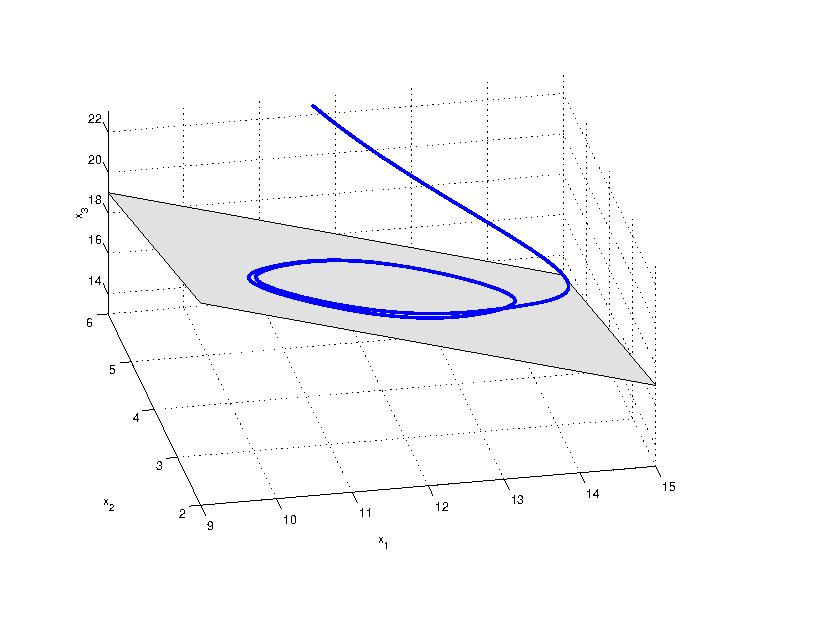
\includegraphics[width=.9\linewidth]{testfig.pdf}
  \caption{Test figure}
  \label{fig:testfig}
\end{figure}

For two-column figures or tables, use the star-form of the
figure/table environment (such as Table~\ref{tab:testtab}). Often, the
double column floats can be used in conjunction with the
\textsf{subfig} package.

Table captions should appear above the table. For better typographical
appearance, avoid vertical lines in the table. Table~\ref{tab:testtab}
shows an example made using the package booktabs.

\begin{table*}[htbp]
  \caption{Test table}
  \label{tab:testtab}
  \centering
  \begin{tabular}{>{\centering}m{2cm} >{\centering}m{2cm}
      >{\centering}m{2cm} >{\centering}m{2cm} >{\centering}m{2cm}
      >{\centering}m{2cm} } \toprule 
      {Initial \\ condition} & \multicolumn{5}{c}{Cost}
      \tabularnewline \cmidrule(r){2-6} 
    & {Algorithm 1} &  {Algorithm 2} & {Algorithm 3} &
      {Algorithm 4} & {Algorithm 5\\The best one} \tabularnewline
      \midrule 
      (-4,0) & 832.72 & 831.72 & 677.89 & 609.44 & 609.39 \tabularnewline
      (-2,.6) &  378.24 & 374.57 & 234.63 & 204.46 & 204.46 \tabularnewline
      \bottomrule
  \end{tabular}
\end{table*}




\section{Mathematics and equations}
\label{sec:math}

For mathematics, use the packacke \textsf{amsmath} (and
\textsf{ams\-symb}). Use the \textsf{align}-environment from
\textsf{amsmath} instead of \textsf{eqnarray},
\begin{align}
  f(x) &= \mathrm{e}^{-x}, \label{eq:e}\\
  g(y) &= \sin^{-1} y. \notag
\end{align}
Note the punctuation. It is also preferable to use the
\textsf{align}-environment for one-line equations, instead of the
\textsf{equation}-environment.

Number those equations which are referred to, such as~(\ref{eq:e}).

One should try to avoid equations that are wider than one column. If
unavoidable, use a float as explained in the \textsf{IEEEtran}\footnote{Can be
  found on \url{http://www.ctan.org/}.} documentation, and place it on
the bottom of a page (use the package \textsf{stfloats}).
See~(\ref{eq:floateqn}) (bottom of page).
\addtocounter{equation}{1} % Account for the floating equation

The equation numbering should still be consequtive,
see~(\ref{eq:multline}). Note that \textsf{amsmath} constructs such as
the \textsf{multline} environment can be used to avoid too wide
equations,
\begin{multline}\label{eq:multline}
  \tilde{V}(x(\infty),\eta(\infty)) - \tilde{V}(x(t_i),\eta(t_i)) \\
  \leq  -\int_{t_i}^{\infty}\!\!\!\!\!\!F(x(\tau),u(\tau;\hat x_0))d\tau
   - \int_{t_i}^{\infty} \!\!\!\! \kappa \|\eta(\tau)\| d \tau.
\end{multline}

\section{Citations}
\label{sec:references}

You should use Harvard reference style, for example using the
bibliography style file \textsf{mic.bst}. Using the package
\textsf{natbib}, cite either in text as shown in~\citet{Hovd04} (using
the \textsf{$\backslash$citet}-command), or in
parantheses~\citep{Hovd92} (using the
\textsf{$\backslash$citep}-command) .  These two first citations are
journal and conference citations, one can also have book
chapter~\citep{Hovd00} or book as in~\citet{Balchen88}, or other
citations.

The file {\tt mic.bst} has been modified to allow DOI information. In the bibliography file
{\tt micartsam.bib} the doi example for \cite{Hallingstad1980} is as follows: {\tt doi = {10.4173/mic.1980.1.1}}.
The MIC class files will automatically add the permanent link to this article in the reference list. We strongly
encourage the use of DOI in the bibliography instead of URL addresses, whenever possible.

\section*{Acknowledgments}

Add, if desired, appropriate acknowledgments here (for example,
financing or any other help).

\bibliographystyle{mic}
\bibliography{micartsam}

\end{document}

